\section{Das Web~2.0}

Um überhaupt die Gründe für eine Weiterentwicklung des Internets in die dezentrale Richtung erläutern und diskutieren zu können, benötigt der Leser oder die Leserin tiefer gehende Informationen über die sowohl technische als auch gesellschaftliche Entwicklung und eine Darstellung der aktuellen Situation, die in den folgenden Kapiteln ausführlicher behandelt werden.


\subsection{Unterschiede zum Web~1.0}

Den genauen Anfang des Internets zu datieren ist kaum möglich, da es bis zur heutigen Verwendung viele Entwicklungen und Meilensteine gegeben hat, die alle in einer eigenen Ausarbeitung Platz finden würden. 
Um nur ein paar Eckdaten zu nennen: Nachdem die Sowjetunion 1957 den ersten Satellit ``Sputnik`` ins All geschossen hat, wurden vor allem in den USA viele Forschungsprojekte vorangetrieben, unter anderem das von der 
\textit{\textbf{A}dvanced \textbf{R}esearch \textbf{P}rojects \textbf{A}gency} 
ins Leben gerufene ARPANET. 
Dieses Netz verknüpfte zunächst vier Computer in verschiedenen amerikanischen Städten und ermöglichte dadurch den In\-for\-ma\-tions\-aus\-tausch~\cite{Krause.2008}. Nach der Umstellung auf das vom amerikanischen Verteidigungsministeriums entwickelte Protokoll \textit{TCP/IP} im Jahr 1983~\cite{Held.2002} stellte es die technische Grundlage für das Internet dar.
Als weitaus wichtiger ist jedoch das Jahr 1991 zu betrachten, genauer den 6. August diesen Jahres. An dem Tag veröffentlichte Tim Berners-Lee seine Vision des WWW, des World Wide Web, an der er zuvor am CERN~
\footnote{
	Die Europäische Organisation für Kernforschung (Conseil Européen pour la Recherche Nucléaire)~\cite{Weltmaschine.de.2019}. Als Physiker und Informatiker arbeitete Berners-Lee an der Möglichkeit des Informationsaustauschs zwischen Wissenschaftlern und Institutionen auf der ganzen Welt~\cite{CERN.2020}.
} 
in der Schweiz gearbeitet hat~\cite{Fiedler.2016}. 

\smallskip

Bis zu diesem Tag interessierte er sich bereits für Hypertext und Verlinkungen, die über den lokalen Rechner hinausgehen, doch er findet kaum Gehör am konservativen und physik-lastigen CERN~\cite{Fiedler.2016}. 
Seine Veröffentlichung in Form der ersten Webseite der Welt schlägt dennoch ein, und er erhält Rückmeldungen aus aller Welt. 
Mit der Verbreitung und dem massentauglichen Einsatz von Computern und Browsern, die auf den grundlegenden Protokollen und Prinzipien von Tim basierten, begann die Phase, die später als Web~1.0 referenziert werden soll. 
Abstrahiert bot das Web in dieser Phase lesenden Zugriff: Durch graphische Oberflächen und das Erstellen von Webseiten ohne Kommandozeilen oder tiefgreifendes technisches Wissen konnten Informationen ins Netz gestellt und durch Hyperlinks miteinander verknüpft werden, auf die eine große Masse von Nutzern Zugriff hatten. 
Als Killer-Applikation dieser Phase gilt der Browser, durch den der Zugriff auf die Seiten ohne technische Hürden und graphisch anschaulich ermöglicht wurde. 
Dabei kamen Webserver zum Einsatz, die als eine Art Speicherort für die Webseiten dienten und diese unter einer spezifischen Adresse für andere Internet-Nutzer zugänglich machten~
\footnote{
	Die erste Website von Tim ist aus historischem Interesse noch immer unter \url{http://info.cern.ch/hypertext/WWW/TheProject.html} erreichbar
}. 
Auch dieser Server wurde von Tim in seiner Zeit am CERN entwickelt. Und obwohl die 2. Phase des Webs viel veränderte und die Techniken weiterentwickelt wurden, blieb dieses grundlegende Konzept bestehen.


\subsection{Technischer Aufbau des Webs}
% ca. 0,5 Seiten

Mit der Zeit wurde das Internet und das WWW immer komplexer, und die technischen Strukturen mit ihnen. 
Es gibt immer mehr Geräte, die an das Internet angebunden sind und daran partizipieren, ebenso wie Anbieter von Webseiten und -diensten. 
Durch die schiere Masse an Geräten und Kommunikation wurden immer mehr Bereiche vernetzt und riesige Rechenzentren errichtet, um mit den derzeitigen Größenordnungen mithalten zu können. 
Das Konzept hinter der Technik jedoch ist relativ simpel und wird Client-Server-Architektur genannt. 
Clients, also die Geräte der Endnutzer, greifen auf Server zu, und damit auf Webseiten oder -dienste der jeweiligen Anbieter, die von den Servern bereitgestellt werden.
Die Kommunikation zwischen Client und Server wird dabei über HTTP realisiert, ein Protokoll, das ebenfalls von Tim Berners-Lee Anfang der 1990er Jahre entwickelt wurde. 
Die Abkürzung steht für \textit{Hyper Text Transfer Protokoll} und beinhaltet grundlegende Regeln, wie die Kommunikation zwischen Netzwerkgeräten vonstatten geht.

\begin{figure*}
	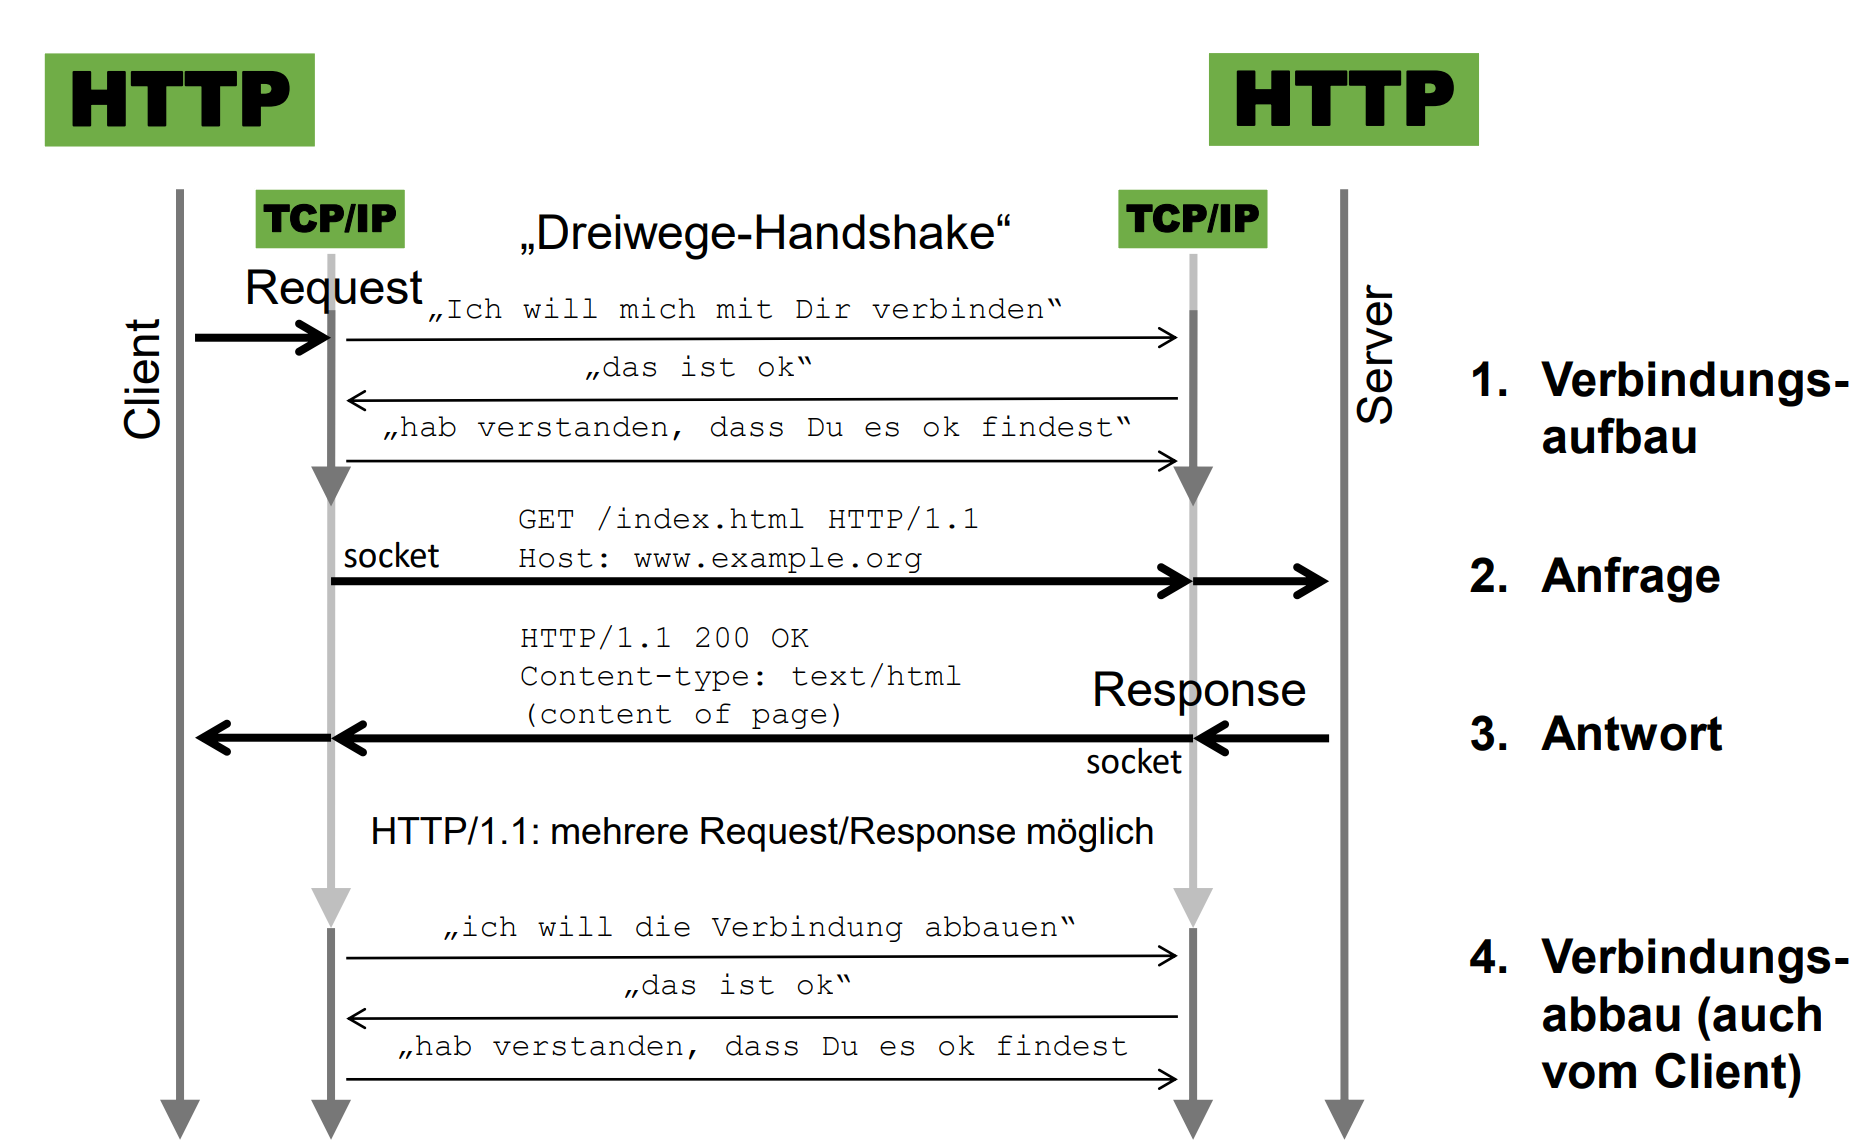
\includegraphics[width=\linewidth]{images/handshake}
	\caption{3-Wege-Handshake bei einem HTTP-Request~\cite{Kneisel.2017}}
	\label{fig:handshake}
\end{figure*}

Im Regelfall schickt ein Client zuallererst eine Anfrage an den Server, um herauszufinden, ob dieser überhaupt bereit ist. 
Ist dies der Fall, antwortet der Server mit einer Erfolgs-Antwort, und der Client kann die benötigte Anfrage stellen. 
Wenn der Server die Bearbeitung fertig gestellt hat, sendet er eine Antwort an den Client, der diese zum Beispiel weiterverarbeiten kann (siehe Figure~\ref{fig:handshake}). 
An dieser Stelle ein Alltagsbeispiel, das wohl jeder Internetnutzer kennt: Eine Google-Suchanfrage. 
Navigiert ein Benutzer beispielsweise auf www.google.de, um eine Google-Suche durchzuführen, wird auf dem Gerät des Nutzers (dem Client) zuerst die Webseite mit der Suchleiste von Google geöffnet. 
Gibt der Nutzer nun "Wie wird das Wetter heute" in die Suchleiste ein und betätigt die Suchen-Schaltfläche, wird eine HTTP-Anfrage an den Server von Google gesendet. 
Ist dieser erreichbar und bereit (was wohl die meiste Zeit der Fall sein dürfte), wird der Such-Term in der HTTP-Anfrage versendet. 
Der Server verwendet nun die Rechenleistung eines Rechenzentrums, um die benötigten Antwortdaten zu "berechnen". 
Dafür benötigt er Metadaten wie beispielsweise den Standort des Clients, der ebenfalls in der HTTP-Anfrage mitgesendet werden kann. Nachdem der Server die Wetterdaten für den jeweiligen Standort abgerufen hat, sendet er eine Antwort, ebenfalls mittels HTTP-Protokoll. Der Client, der auf diese Antwort gewartet hat, kann die Informationen nun graphisch aufbereiten und auf dem Display des Nutzers darstellen.
% Statistik: Anzahl Requests/Responses am Tag bzw. Datenmenge
% Überleitung
Dieses Konzept ist zwar in den Jahren entsprechend der Gerätezahl und der HTTP-Kommunikation mit skaliert, stößt jedoch in einigen Punkten an seine Grenzen. An manchen Stellen birgt es sogar große Probleme. Und wenn man sich mit der Kritik am Web~2.0 befasst, sind technische Gegebenheiten nicht immer das Problem, in vielen Fällen aber die Ursache, weshalb die Rufe nach Dezentralisierung lauter werden.
% Beleg
Aufgrund dessen spielt das Verständnis der dem Internet zugrunde liegenden Technik mindestens aus konzeptioneller Sicht eine nicht unerhebliche Rolle.


%\subsection{Aktuelle Situation}
% ca. 0,5 Seiten

% Entwicklung seit der Dotcom-Blase (was macht die Phase Web~2.0 aus):
%	- bunteres Web
%	- Partizipation von Nutzern
% TBLee: Mag Begriff Web~2.0 nicht
% Plattformen als "Mittelsmänner", denen Vertraut werden muss (+ Beispiele)


\subsection{Kritik und Problematik}
% ca. 3 Seiten

Doch nun zu den Gründen, warum es überhaupt Menschen gibt, die sich mit dem Einsatz von neuen Techniken in der nächsten Generation des Internets beschäftigen. Wie bereits erwähnt hat sich das Internet schnell sehr stark entwickelt, um nicht zu sagen verändert. Dennoch basiert das grundlegende technische Konzept auf den Anfang der neunziger Jahre erfundenen Webservern. Doch wieso ist das schlecht, es funktioniert doch alles, oder? 
Diese Aussage ist theoretisch richtig, doch durch diese Struktur entstehen Probleme, die nicht auf den ersten Blick sichtbar sind und die viel zu lange inkonsequent behandelt wurden. Um das gewichtigste Problem an den Anfang zu stellen: Die Kontrolle über die eigenen Daten. Durch die im vorhergehenden Kapitel beschriebenen Plattformen, die als "Mittelsmann" dienen, ist es den Nutzern nahezu unmöglich, Einfluss auf die Speicherung und Verarbeitung der eigenen Daten zu nehmen. Die einzige Möglichkeit ist in den meisten Fällen, auf die Nutzung dieser Dienste oder sogar des gesamten Internets zu verzichten, was in der heutigen Zeit kaum möglich und auch nicht im Sinne des Erfinders ist.
% Kampf von Berners-Lee für freies Internet irgendwo erwähnen
Zudem hat sich die Nutzung von Internet-Plattformen herauskristallisiert, hinter denen riesige Tech-Konzerne stehen, die international agieren und sich geschickt in der Umgehung von lokalen Gesetzen und Auflagen anstellen. Informationen über die Datenverarbeitung sind oft intransparent in seitenlangen Impressen versteckt, sodass diese einfach überlesen werden. Und selbst wenn man sich die Mühe des Entschlüsselns macht, hat man in der Regel keine Wahl: Man vertraut der Plattform mit der Nutzung die eigenen Daten an, oder eben nicht.
% Beispiele für Tech-Giganten und Datenschutzbedenken

Das Unternehmen muss dabei nicht einmal selbst die Daten verkaufen, vermutlich ist dies ziemlich selten der Fall. Dennoch gibt es Andere, die das tun: Meldungen zu Datenschutzskandale in Form von geleakten oder gehackten Daten häufen sich. Zum Teil kursieren Datensätze mit Millionen von Nutzerdaten frei verkäuflich im Internet!
% Belege!

Dies kann nur geschehen, wenn die Systeme der Anbieter nicht ausreichend geschützt sind. Doch Hacker werden immer kreativer, und vor allem für kleinere Plattformen ist es schwierig, die Schutzmechanismen auf dem neuesten Stand zu halten. 
Ein Grund für den Erfolg solcher Datendiebstähle ist, dass die Server in der beschriebenen CS-Struktur sogenannte SPOF's darstellen. Dies steht für \textit{Single Point of Failure} und beschreibt in einem Hardware-System eine Komponente, ohne die das gesamte System nicht Betriebsbereit ist. Das Internet fällt zwar nicht aus, weil eine einzige Webseite offline ist, dennoch kann der Ausfall von verschiedenen Diensten und Plattform verheerende Folgen haben. Diese Ausfälle können sowohl durch Cyber- (oder sogar physischen) Angriffen als auch technischen Defekten entstehen. Diese können in beiden Fällen aufwendig zu Beheben sein und dadurch stundenlange Ausfälle verursachen. Bei Social-Media-Plattformen mag das keine verheerenden Auswirkungen haben, doch es gibt mittlerweile viele kritische Systeme, die ans Internet angeschlossen sind, und von denen zum Teil Leben abhängen.
% Beispiele

\smallskip

\textsc{Recap} Abschließend die größten Probleme des Web~2.0 und damit die Gründe für ein dezentrales Internet zusammengefasst:
\begin{itemize}
	\item Server stellen SPOF's dar, Ausfälle oder Attacken können verheerende Folgen haben
	\item Cyber-Attacken können in Datendiebstählen resultieren, Datensätze werden im Darknet an den meistbietenden verkauft
	\item Der gewöhnliche Verbraucher hat keine Einsicht in die eigenen Daten, geschweige denn die Kontrolle darüber
\end{itemize}

% Stateless einfügen!

\smallskip





